\section{A linguagem do Wiring}

O Wiring é uma API (Application Programming Interface) da linguagem Processing, mantendo a ideia inicial de facilidade na aprendizagem e aplicação visual. 
\subsection{IDE }

O ambiente de fiação (Integrated Development Environment ou IDE) possui um editor de texto e um compilador para escrever programas para o hardware Wiring. 

\begin{figure}[htb]
	\caption{\label{wiringIDE}Ambiente de Desenvovlimento do Wiring}
	\begin{center}
	    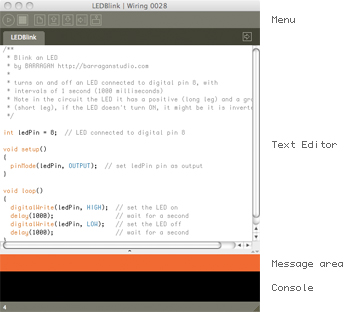
\includegraphics[scale=0.9]{artigo/refs/ide.jpeg}
	\end{center}
	%\legend{Fonte: Site da 3GPP}
\end{figure}

\subsection{A biblioteca Wiring no Arduíno}
\subsubsection{Principais Funções}

%Eu (Ricardo) faço de boa